\documentclass[12pt]{article}

\usepackage[T1]{fontenc}
\usepackage[utf8]{inputenc}
\usepackage{listings}
\usepackage{amssymb}
\usepackage{amsmath}
\usepackage{amsthm}
\usepackage{etexcmds}
\usepackage{thmtools}
\usepackage{tikz-cd}

%lean highlight
\usepackage{color}
\definecolor{keywordcolor}{rgb}{0.7, 0.1, 0.1}   % red
\definecolor{tacticcolor}{rgb}{0.0, 0.1, 0.6}    % blue
\definecolor{commentcolor}{rgb}{0.4, 0.4, 0.4}   % grey
\definecolor{symbolcolor}{rgb}{0.0, 0.1, 0.6}    % blue
\definecolor{sortcolor}{rgb}{0.1, 0.5, 0.1}      % green
\definecolor{attributecolor}{rgb}{0.7, 0.1, 0.1} % red

\def\lstlanguagefiles{lstlean.tex}
% set default language
\lstset{language=lean}

% theorem style
\theoremstyle{definition}
\newtheorem{theorem}{Theorem}[section]
\newtheorem{proposition}[theorem]{Proposition}
\newtheorem{lemma}[theorem]{Lemma}
\newtheorem{corollary}[theorem]{Corollary}
\newtheorem{definition}[theorem]{Definition}
\theoremstyle{remark}
\newtheorem*{remark}{Remark}

% Remove blueprint commands
\newcommand{\uses}[1]{}
\newcommand{\proves}[1]{}
\newcommand{\discussion}[1]{}
\newcommand{\lean}[1]{}
\newcommand{\leanok}{}
\newcommand{\mathlibok}{}
\newcommand{\notready}{}

%Notaion
\newcommand{\dist}{\text{ dist }}
\newcommand{\N}{\mathbb{N}}
\newcommand{\R}{\mathbb{R}}
\newcommand{\C}{\mathbb{C}}

%Tikz arc 
\tikzset{
            carc/.style args={#1:#2:#3}{
              insert path={+(#1:#3) arc (#1:#2:#3)}
            }
          }

\title{Formalisation of constructible numbers}
\author{Ludwig Monnerjahn}
%\date{\time}

\begin{document}

\maketitle

This talk is about formalising the proof that the set of all constructible points $\mathcal{M}_{\infty}$ forms a field. 
This is the first step needed to solve ancient construction problems, such as doubling the cube and trisecting an angle. 
$\mathcal{M}_{\infty}$ is a subset of the complex numbers $\mathbb{C}$. So, we just need to show that $\mathcal{M}_{\infty}$ is a subfield of $\mathbb{C}$. 
In lean we do this by defining a structure on $\mathcal{M}_{\infty}$.

\begin{lstlisting}
    noncomputable def MFinf : Subfield ℂ where
        carrier := _
        zero_mem' := _
        one_mem' := _
        add_mem' := _
        neg_mem' := _
        mul_mem' := _
        inv_mem' := _
\end{lstlisting}

Now we need to fill in the blanks. To do this we first need to fill in the carrier set of $\mathcal{M}_{\infty}$, 
so we need to recall the definitions for $\mathcal{M}_{\infty}$ and state them in lean.

\section{Definition of $\mathcal{M}_{\infty}$}
We start with a basic set of points $\mathcal{M} \subseteq \mathbb{C}$ in the complex plane. 
Without loss of generality we can assume that $\mathcal{M}$ contains the points $0$ and $1$.
Because constructing whit less than two points is trivial and we can always scale and translate the plane to get $0$ and $1$ in $\mathcal{M}$.

\begin{definition}[Line]
    \label{def:line}
    A line $l$ through two points $x,y\in\mathbb{M}$ for $x\ne y$ is defined by the set: $$l:=\{\lambda x+(1-\lambda)y\mid\lambda\in\mathbb{R}\}.$$
\end{definition}

\begin{lstlisting}
    structure line where
        (z₁ z₂ : ℂ)

    def line.points (l: line) : Set ℂ:= {(t : ℂ) * l.z₁ + (1-t) * l.z₂ | (t : ℝ)}
\end{lstlisting}

\begin{definition}[Circle]
    \label{def:circle}
    A circle $c$ with center $z\in\mathbb{C}$ and radius $r\in\mathbb{R}_{\ge 0}$ is defined by the set: $$c:=\{z\in\mathbb{C} \mid\|z-c\|=r\}.$$
\end{definition}

\begin{lstlisting}
    structure circle where
        (c : ℂ)
        (r : ℝ)

    def circle.points (c: circle) := Metric.sphere c.c c.r
\end{lstlisting}


\begin{definition}[Set of lines]
    \label{def:set_of_lines_and_circles}
    $\mathcal{L(M)}$ is the set of all real straight lines defined by two points in $\mathcal{M}$.\\
    And $\mathcal{C(M)}$ is the set of all circles defined by a centre in $\mathcal{M}$ and a radius equal to the distance between two points in $\mathcal{M}$.
\end{definition}

\begin{lstlisting}
    def set_of_lines (M : Set ℂ) : Set (line) := {l | ∃ x y ∈ M, l = line.mk x y}
    def C (M:Set ℂ): Set circle := {c |∃ z r₁ r₂, c = {c:=z, r:=(dist r₁ r₂)} ∧ z ∈ M ∧ r₁ ∈ M ∧ r₂ ∈ M}
\end{lstlisting}

\begin{definition}[Ruels to construct a point]
    \label{def:rules_to_constructed_a_point}
    We define operations that can be used to construct new points.
    \begin{enumerate}
        \item $(ILL)$ is the cut of two lines in $\mathcal{L(M)}$.
        \item $(ILC)$ is the cut of a line in $\mathcal{L(M)}$ and a circle in $\mathcal{C(M)}$.
        \item $(ICC)$ is the cut of two circles in $\mathcal{C(M)}$.
    \end{enumerate}
    $ICL(\mathcal{M})$ is the set $\mathcal{M}$ combiened of all points that can be constructed using the operations $(ILL)$, $(ILC)$ and $(ICC)$ and $\mathcal{M}$.
\end{definition}

\begin{lstlisting}
    def ill (M:Set ℂ): Set ℂ := { z  |∃l₁ ∈ L M, ∃ l₂ ∈ L M,  z ∈ l₁.points ∩ l₂.points}
    def ilc (M:Set ℂ): Set ℂ := { z  |∃c ∈ C M, ∃ l ∈ L M,  z ∈ c.points ∩ l.points}
    def icc (M:Set ℂ): Set ℂ := { z  |∃c₁ ∈ C M, ∃ c₂ ∈ C M,  z ∈ c₁.points ∩ c₂.points}

    def ICL_M (M : Set ℂ) : Set ℂ := M ∪ ill M ∪ ilc M ∪ icc M
\end{lstlisting}

\begin{definition}[Set of constructable points]
    \label{def:set_of_constructable_points}
    We define inductively the chain
    \begin{equation*}
        \mathcal{M}_0 \subseteq \mathcal{M}_1 \subseteq \mathcal{M}_2 \subseteq \dots
    \end{equation*}
    with $\mathcal{M}_0 = \mathcal{M}$ and $\mathcal{M}_{n+1} = ICL(\mathcal{M}_n)$.\newline
    And call $\mathcal{M}_{\infty} = \bigcup_{n \in \mathbb{N}} \mathcal{M}_n$ the set of all constructable points.
\end{definition}

\begin{lstlisting}
    def M_I (M : Set ℂ) : ℕ → Set ℂ
        | 0 => M
        | (Nat.succ n) => ICL_M (M_I M n)

    def M_inf (M : Set ℂ) : Set ℂ :=  ⋃ (n : ℕ), M_I M n
\end{lstlisting}

We can now fill in the firtst blank:
\begin{lstlisting}
    noncomputable def MFinf (M: Set ℂ) : Subfield ℂ := {
    carrier := M_inf M
\end{lstlisting}

\section{Zero and one in $\mathcal{M}_{\infty}$}
And since we assume that $\mathcal{M}$ contains the points $0$ and $1$ we can fill in the next two blank, 
after proving that $\mathcal{M} \subseteq \mathcal{M}_{\infty}$.

\begin{lemma}[$\mathcal{M}$ in $\mathcal{M}_i$]
    \label{lem:M_in_Mi}
    The set $\mathcal{M}$ is in $\mathcal{M}_i$, i.e. $$\mathcal{M} \subseteq \mathcal{M}_i.$$
\end{lemma}
\begin{proof}
    Combeing the fact that $\mathcal{M}_0 = \mathcal{M}$ \ref{def:set_of_constructable_points} and the monotonity of $\mathcal{M}_i$ wich sollos by $\mathcal{M} \subset \mathcal{ICL(M)}$.
\end{proof}

\begin{lstlisting}
    lemma M_in_ICL_M (M : Set ℂ) : M ⊆ ICL_M M := by
        unfold ICL_M
        intro x hx 
        left; left; left
        exact hx

    lemma M_I_Monotone (M : Set ℂ) : ∀n, M_I M n ⊆ M_I M (n+1) := by
        intro n
        apply M_in_ICL_M

    lemma M_in_M_I (M : Set ℂ) : ∀n, M ⊆ M_I M n := by
        intro n
        induction n
        simp only [M_I]
        exact fun ⦃a⦄ a => a
        case succ n hn =>
          apply le_trans hn
          apply M_I_Monotone
\end{lstlisting}

\begin{lemma}[$\mathcal{M}_i$ in $\mathcal{M}_{\infty}$]

    The set $\mathcal{M}_i$ is in $\mathcal{M}_{\infty}$, i.e. $$\mathcal{M}_i \subseteq \mathcal{M}_{\infty}.$$
\end{lemma}
\begin{proof}
    Follows from the definition of $\mathcal{M}_{\infty}$.
\end{proof}

\begin{lstlisting}
    lemma M_I_in_M_inf (M : Set ℂ)(m: ℕ): M_I M m ⊆ M_inf M := by
        unfold M_inf
        exact Set.subset_iUnion_of_subset m fun ⦃a⦄ a => a
\end{lstlisting}

\begin{lemma}[$\mathcal{M}$ in $\mathcal{M}_{\infty}$]

    The set $\mathcal{M}$ is in $\mathcal{M}_{\infty}$.
\end{lemma}
\begin{proof}
    \uses{lem:M_i_in_M_inf, lem:M_in_Mi}
    Combeing $\mathcal{M} \subseteq \mathcal{M}_i$ \ref{lem:M_in_Mi} and $\mathcal{M}_i \subseteq \mathcal{M}_{\infty}$ \ref{lem:M_i_in_M_inf} we get the result.
\end{proof}

\begin{lstlisting}
    lemma M_M_inf (M : Set ℂ) : M ⊆ M_inf M := by apply le_trans (M_in_M_I M 0) (M_I_in_M_inf M 0)
\end{lstlisting}

So now we have:
\begin{lstlisting}
    noncomputable def MField (M: Set ℂ)(h₀: 0 ∈ M)(h₁: 1∈ M): Subfield ℂ := {
        carrier := M_inf M
        zero_mem' := by exact M_M_inf M h₀
        one_mem' := by exact M_M_inf M h₁
\end{lstlisting}
\section{Construction}
To fill in the rest, we need to construct addition, multiplication, negation and inversion of constructable numbers.
In the followuing chapter the proof shema is given by construct lines and such that the wanted point is there intersection. Thefore aren't in the handout just the constructionn.
The full proofs can be would in the Blueprint.

\begin{lemma}[Addition of complex numbers]
    \label{lem:construction_add}
    For $z_1, z_2 \in M_{\infty}$ is $z_1 + z_2 \in M_{\infty}$.
\end{lemma}
This constrution is teken from \cite{JAN_SCHROEER:2023}.\\
One can construct the point $z_1 + z_2$ by drawing a circle with center $z_1$ and radius $\|z_2\|$ and a circle with center $z_2$ and radius $\|z_1\|$ and taking the intersection of the two circles.\ref{Fig.2}

\begin{figure}[h!]
    \centering
    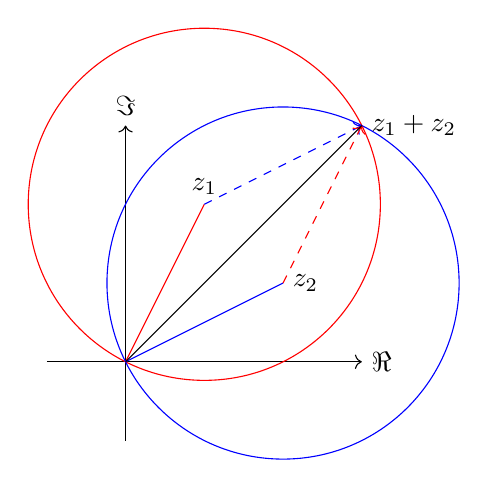
\begin{tikzpicture}
        \draw[->] (-1,0) -- (3,0) node[right] {$\Re$};
        \draw[->] (0,-1) -- (0,3) node[above] {$\Im$};
        \draw (0,0) -- (1,2) node[above] {$z_1$}[red];
        \draw (0,0) -- (2,1) node[right] {$z_2$}[blue];
        \draw (1,2) circle (2.2360679775)[red];
        \draw (2,1) circle (2.2360679775)[blue];
        \draw[dashed,->] (1,2) -- (3,3)[blue];
        \draw[dashed,->] (2,1) -- (3,3)[red];
        \draw (0,0) -- (3,3) node[right] {$z_1 + z_2$};
    \end{tikzpicture}
    \caption{Construction of $z_1 + z_2$}
    \label{Fig.2}
\end{figure}

\begin{lstlisting}
    lemma add_M_Inf (M: Set ℂ) (h₀: (0:ℂ)∈ M) (z₁ z₂ : ℂ) (hz₁ : z₁ ∈ (M_inf M)) (hz₂ : z₂ ∈ (M_inf M)):
            z₁ + z₂ ∈ (M_inf M) := by
        let c₁ : Construction.circle := {c := z₁, r := (dist 0 z₂)}
        let c₂ : Construction.circle := {c := z₂, r := (dist 0 z₁)}
        have hc₁ : c₁ ∈ C (M_inf M) := by
            use z₁, 0, z₂
            refine ⟨?_, (by exact hz₁), (by exact M_M_inf M h₀), (by exact hz₂)⟩
            simp [c₁]
        have hc₂ : c₂ ∈ C (M_inf M) := by
            use z₂, 0, z₁
            refine ⟨?_, (by exact hz₂), (by exact M_M_inf M h₀), (by exact hz₁)⟩
            simp [c₂]
        apply icc_M_inf M
        refine ⟨c₁, (by exact hc₁), c₂, (by exact hc₂), ?_⟩
        simp [circle.points, Set.mem_inter_iff]
\end{lstlisting}

\begin{lemma}[Negative complex numbers]
    \label{lem:construction_neg}
    \lean{z_neg_M_inf}
    \leanok
    \uses{def:set_of_constructable_points}
    For $z \in M_{\infty}$ is $-z \in M_{\infty}$.
\end{lemma}
This constrution is teken from \cite{JAN_SCHROEER:2023}.\\
To get the point $-z$ we can use the second intersection of the line through $0$ and $z$ with circle with center $0$ and radius $\|z\|$.\ref{Fig.1}

\begin{figure}[h!]
    \centering
    \begin{tikzpicture}
        \draw[->] (-1,0) -- (3,0) node[right] {$\Re$};
        \draw[->] (0,-1) -- (0,3) node[above] {$\Im$};
        \draw (0,0) -- (2,2) node[right] {$z$};
        \draw (0,0) -- (-2,-2) node[left] {$-z$};
        \draw (0,0) circle (2.8);
    \end{tikzpicture}
    \caption{Construction of $-z$}
    \label{Fig.1}
\end{figure}

\begin{lstlisting}
    lemma z_neg_M_inf (M: Set ℂ) (h₀: (0:ℂ)∈ M) (z : ℂ) (hz : z ∈ (M_inf M)) : -z ∈ (M_inf M) := by
        by_cases z0:(z=0)
        . simp [z0, M_M_inf M h₀]
        let l : line := {z₁ := 0, z₂ := z}
        let c : Construction.circle := {c := 0, r := (dist 0 z)}
        have hl : l ∈ L (M_inf M) := by
            use 0, z
            refine ⟨?_, (by apply M_M_inf M h₀), (by exact hz), ?_⟩
            simp only [l]
            simp  [eq_comm, z0]
        have hc : c ∈ C (M_inf M) := by
            use 0, 0, z
            refine ⟨?_, (by exact M_M_inf M h₀), (by exact M_M_inf M h₀), (by exact hz)⟩
            simp [l, c]
        apply ilc_M_inf M
        refine ⟨c , (by exact hc), l, (by exact hl), ?_⟩
        simp [circle.points, line.points]
        use 2
        push_cast
        ring_nf
\end{lstlisting}

\begin{lemma}[Multiplication of positve real numbers]
    \label{lem:construction_mul}
    \lean{ab_in_M_inf}
    \leanok
    \uses{def:set_of_constructable_points}
    For $a, b \in M_{\infty}\cap\R$ is $a \cdot b \in M_{\infty}$.
\end{lemma}
This constrution is taken from \cite{cox2012galois}.\\
To get the point $a\cdot b$ we draw a line trough $a$ and $\imath$ and a parallel line through $\imath b$. The intersection of the second line with the real axis is $a\cdot b$.\ref{Fig.5} 

\begin{figure}[h!]
    \centering
    \begin{tikzpicture}
        \draw[->] (-0.5,0) -- (5,0) node[right] {$\Re$};
        \draw[->] (0,-0.5) -- (0,3) node[above] {$\Im$};
        \coordinate[label=135:$\imath$] (i) at (0,1);
        \coordinate[label=-90:$a$] (a) at (2,0);
        \coordinate[label=135:$\imath b$] (ib) at (0,2);
        \coordinate[label=-90:$ab$] (ab) at (4,0);
        \fill[black] (i) circle (2pt);
        \fill[black] (a) circle (2pt);
        \fill[black] (ib) circle (2pt);
        \fill[black] (ab) circle (2pt);
        \draw (a) -- (i);
        \draw (ib) -- (ab);
    \end{tikzpicture}
    \caption{Construction of $z_1 \cdot z_2$}
    \label{Fig.5}
\end{figure}

\begin{corollary}[Multiplication of complex numbers]
    \label{cor:construction_mul_complex}
    %\lean{mul_in_M_inf}
    %\leanok
    \uses{def:set_of_constructable_points}
    For $z_1, z_2 \in M_{\infty}$ is $z_1 \cdot z_2$ in $M_{\infty}$.
\end{corollary}
\begin{proof}
    \uses{lem:construction_mul, lem:construction_add, cor:construction_sub, lem:construction_real, lem:construction_imag}
    Let $z_1 = a + \imath b$ and $z_2 = c + \imath d$. Then $$z_1 \cdot z_2 = (a + \imath b) \cdot (c + \imath d) = (a \cdot c - b \cdot d) + \imath (a \cdot d + b \cdot c).$$
    By combeing the Lemmas \ref{lem:construction_mul}, \ref{lem:construction_add}, \ref{cor:construction_sub}, \ref{lem:construction_real} and \ref{lem:construction_imag} we get that $z_1 \cdot z_2 \in M_{\infty}$.
\end{proof}


\begin{lemma}[Invers of a pos real number]
    \label{lem:construction_inv}
    \lean{ainv_in_M_inf}
    \leanok
    \uses{def:set_of_constructable_points}
    If $a \in M_{\infty}\cap\R$, then $a^{-1}$ is in  $M_{\infty}$.
\end{lemma}

This can be construceted analog to the multiplication of positve real numbers. Usind the fact that $a\cdot a^{-1} = 1$. Draw a line through $1$ and $\imath a$ and a parallel line through $\imath$. The intersection of the second line with the real axis is $a^{-1}$.\ref{Fig.6}
\begin{proof}
    \uses{def:line, def:set_of_lines, lem:ill_M_inf, lem:construction_imath_r, cor:construction_imath, lem:construction_add, cor:construction_sub}
    The proof is analog to the proof of Lemma \ref{lem:construction_mul} we just need two lines $l = \{1-\imath z + \imath, \imath\}$ and $l_{\Re} = \{1,0\}$.\\
    With  out loss of generality we can assume that $a \ne 0$.\\
    That there are in $\mathcal{L(M_{\infty})}$ follows analog to the proof of Lemma \ref{lem:construction_mul}.\\ 
    So we have just to show that $z^{-1} \in l$, i.e. $\exists t: t  (1 - \imath a + \imath) + (1 - t)  I = a^{-1}$ $$t  (1 - \imath a + \imath) + (1 - t)  \imath \stackrel{t:=a^{-1}}{=}  a^{-1} - a^{-1} \imath a + a^{-1}\imath + \imath - a^{-1}\imath = a^{-1}.$$
    The rest follws analog.
\end{proof}
\begin{figure}[h!]
    \centering
    \begin{tikzpicture}
        \draw[->] (-1,0) -- (2,0) node[right] {$\Re$};
        \draw[->] (0,-1) -- (0,3) node[above] {$\Im$};
        \coordinate[label=135:$\imath$] (i) at (0,1);
        \coordinate[label=-90:$1$] (1) at (1,0);
        \coordinate[label=135:$\imath a$] (ia) at (0,2);
        \coordinate[label=-90:$a^{-1}$] (ainv) at (0.5,0);
        \fill[black] (i) circle (2pt);
        \fill[black] (1) circle (2pt);
        \fill[black] (ia) circle (2pt);
        \fill[black] (ainv) circle (2pt);
        \draw (1) -- (ia);
        \draw (i) -- (ainv);
    \end{tikzpicture}
    \caption{Construction of $z^{-1}$}
    \label{Fig.6}
\end{figure}

\begin{corollary}[Invers of a complex number]
    \label{cor:inv_M_inf}
    \lean{inv_M_inf, z_inv_eq}
    \leanok
    \uses{def:set_of_constructable_points}
    If $z \in M_{\infty}$, then $z^{-1}$ is in  $M_{\infty}$.
\end{corollary}
\begin{proof}
    \uses{lem:construction_inv, lem:construction_mul, cor:construction_sub, lem:construction_real, lem:construction_imag, lem:construction_add}
    For $z \in M_{\infty}$ we can write $z = a + \imath b$ with $a, b \in \R$. Then
    $$z^{-1} = \frac{1}{z} = \frac{\overline{z}}{z\overline{z}} = \frac{a - \imath b}{a^2+b^2}= (a - \imath b) \cdot (aa+bb)^{-1}.$$
    Now we can again combiened the lemmas for addition\ref{lem:construction_add}, subtraction\ref{cor:construction_sub}, multiplication\ref{cor:construction_mul_complex} and the corollary for the invers of a positive real number\ref{lem:construction_inv} with the exists of real an imaginary\ref{construction_re_im} part to get that $z^{-1} \in M_{\infty}$.
\end{proof}
\section{Conclusion}

At last, we have assembled the requisite elements for the construction of the field of constructible numbers $\mathcal{M}_{\infty}$.
\begin{lstlisting}
    noncomputable def MField (M: Set ℂ)(h₀: 0 ∈ M)(h₁: 1∈ M):
            Subfield ℂ where
        carrier := M_inf M
        zero_mem' := by exact M_M_inf M h₀
        one_mem' := by exact M_M_inf M h₁
        add_mem' := by apply add_M_Inf M h₀
        neg_mem' := by apply z_neg_M_inf M h₀
        mul_mem' := by apply mul_M_inf M h₀ h₁
        inv_mem' := by apply inv_M_inf M h₀ h₁
\end{lstlisting}

Now it is just an \verb|instance|, proven by \verb|exact?|. To get the structure of the field. Normally this would be done by \verb|infer_instance|, but I want to show the proof in this talk.
\begin{lstlisting}
    noncomputable instance MField_field (M: Set ℂ)(h₀: 0 ∈ M)
            (h₁: 1∈ M): Field (MField M h₀ h₁) := by
        exact SubfieldClass.toField (Subfield ℂ) (MField M h₀ h₁)
\end{lstlisting}

This can be used to proof that $x\in \mathbb{C}$ is in $\mathcal{M}_{\infty}$ if and only if the degree of $x$ over $\mathbb{Q}(M)$ is of the form $2^n$ for some $n\in \mathbb{N}$.

\bibliographystyle{plain}
\bibliography{reference}

\nocite{*}

\end{document}